When a correction is added in the dynamical system, it needs to influence trajectories that initially went through. The trajectory \emph{should not} simply go straight forward, and when reaching a correction, following it, see \autoref{bad_example}. It should anticipate and slowly get around of it in advance in order to have a smooth result, see \autoref{gpr_example}. For this non-linear application, Gaussian Process regression is selected.

\subsection{Motivation}

\begin{figure}[H]
\centering
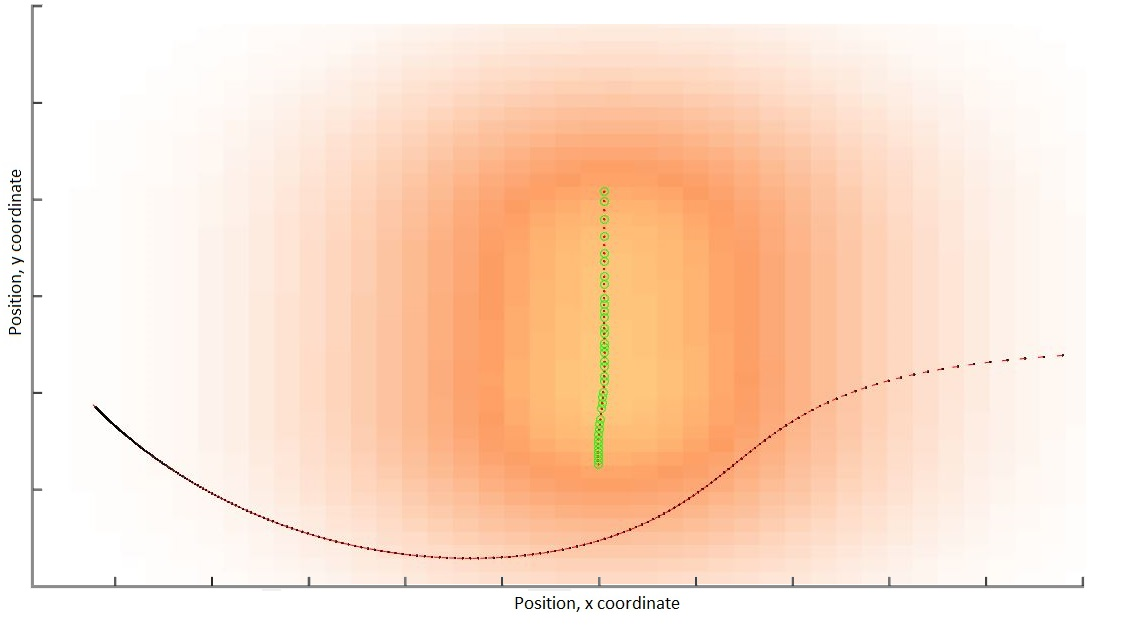
\includegraphics[width=10cm]{img/gpr_ex_unzoom.jpg}
\caption{Example of a trajectory that get around a correction. Green circles are the discrete correction, black dot points the trajectory, the red arrows the normalized velocity of each dot and red-orange gradient the amplitude of the influence of the correction.}
\label{gpr_example}
\end{figure}

\begin{figure}[H]
 \centering
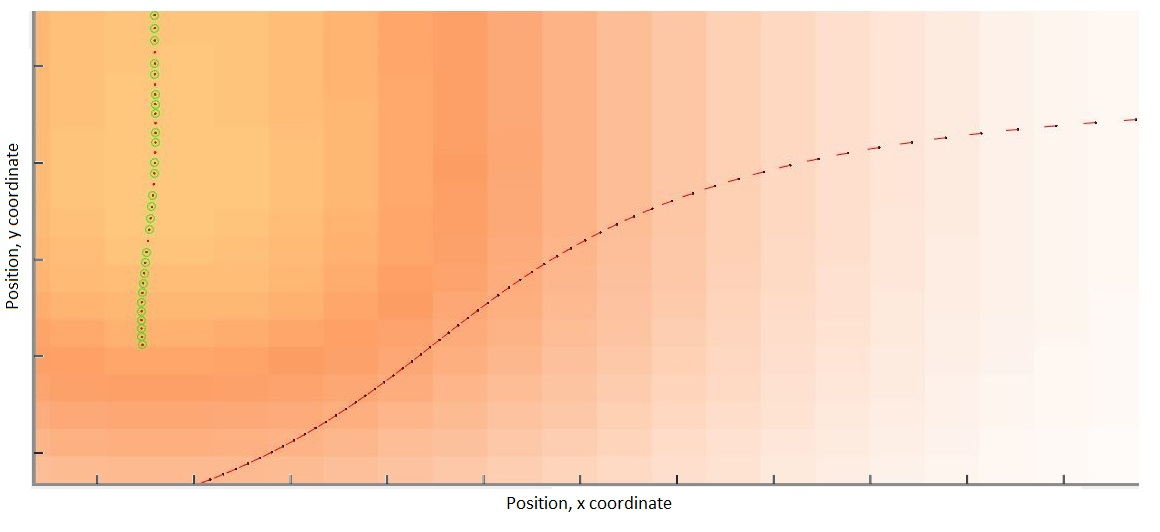
\includegraphics[width=10cm]{img/gpr_ex.jpg}
\caption{Zoom of \autoref{gpr_example} system. Example of a trajectory that gets around a correction. Green circles are the discrete correction, black dot points the trajectory, the red arrows the normalized velocity of each dot and red-orange gradient the amplitude of the influence of the correction.}
\end{figure}

As we can see, the correction needs to get around the correction without simply reaching it and then following it until reaching the attractor, see a bad example in \autoref{bad_example};

\begin{figure}[H]
\centering
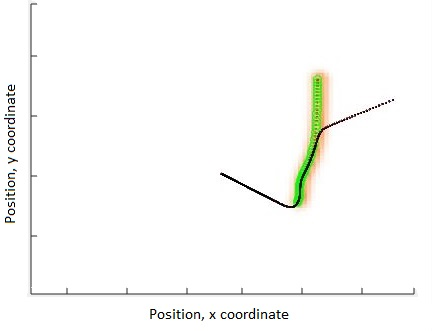
\includegraphics[width=10cm]{img/bad_example.jpg}
\caption{Bad example of avoiding correction.\\\hspace{0cm}The trajectory do not get around, it simply follow it. Green circles are the discrete correction, black dot points the trajectory, the red arrows the normalized velocity of each dot.}
\label{bad_example}
\end{figure}

GPs are used in our application because they encapsulate the property that proximity points have more impact than distant points.

%section 2 : Review on standard GPR --------------------
\subsection{Quick review on standard GPR}

Gaussian Process Regression is a very popular tool for nonlinear regression problems. This tunable algorithm makes powerful and robust applications. However, its biggest drawback is the quadratic computational complexity. Indeed, GPR involves the inversion of an $N \times N$ matrix, where $N$ is the number of training points. That's why this tool becomes relatively slow for application
with more than a few thousand of training points in real time.\\

\subsubsection{Definition}

The Gaussian Process Regression works by computing estimated data in a defined space. It takes as an input training points and observed value (the training points represent the location of the observed value, there are as many training points as estimated value), and testing points. It returns estimated value at the location of the testing points. Let 
$\{\vecc{x_i}\}_{i=1}^N$ be a set of $N\ D$-dimensional training input vectors $\vecc{x_i} \in \real^D$ and its associated observed value $\{y_i\}_{i=1}^N$ with $y_i \in \real$ for all $i=1\hdots N$.\\
The GPR works using a covariance function 
$f(x_i, x_j)$ and a covariance matrix $\mat K$ defined as:

\begin{equation}
  \label{equ_covariancetrainingdata}
  \mat K =
  \begin{bmatrix}
    k(\vecc x_1, \vecc x_1) & \hdots & k(\vecc x_1, \vecc x_N) \\ 
    \vdots & \ddots & \vdots \\ 
    k(\vecc x_N, \vecc x_1) & \hdots & k(\vecc x_N, \vecc x_N) \\ 
  \end{bmatrix}
\end{equation}

\subsubsection{Joint distribution}

Assuming a mean of 0 and a variance of $\sigma_n^2$, the joint distribution of the observed output is:

\begin{equation}
  \label{equ_probdist}
  p(\vecc y) = \mathcal{N}(\vecc 0, \mat K + \sigma_n^2 \mat I)
\end{equation}

where $\vecc y = [y_1,\hdots, y_N]^T$ are the observed values. We assume that the outputs are independent of their observed values, indeed the covariance function only depends on the input.\\

By extending our distribution to a $x^*$ testing point and its associated $y^*$ observed value, the distribution becomes:

\begin{equation}
  \label{equ_probdist2}
  p\left(
    \begin{bmatrix}
      \vecc y \\ y^*
    \end{bmatrix}
\right) = \mathcal{N}\left(\vecc 0,
\begin{bmatrix}
  \mat K & \vecc k^* \\ \vecc k^{*T} & k(x^*, x^*)
\end{bmatrix}
+ \sigma_n^2 \mat I\right)
\end{equation}

where $\vecc k^* = [k(x_1, x^*), \hdots, k(x_N, x^*)]^T$. This Gaussian process will predict $y^*$ using \autoref{equ_probdist2}. Standard Gaussian conditioning yields:

\begin{equation}
  \label{equ_GPR}
  p(y^* | \vecc y) =  \mathcal{N}(\mu^*, c^*)
\end{equation}
with known forms of $\mu^*$ and $c^*$. For brevity, we only write the form for $ \mu^*$:

\begin{equation}
  \label{equ_mustrar}
  \mu^* = \vecc k^{*T}(\mat K + \sigma_n^2 \mat I)^{-1}\vecc y
\end{equation}

The result equation needs an inversion of a $N \times N$ matrix, this is the main problem of computational cost of GPR.

\subsubsection{GPR influences of the correction}

In our application, see \autoref{gpr_example}, the correction is composed by training points ($x_i$), the angle between the velocity of each points of the correction and the original trajectory at those points are the observed values ($y_i$ values) and the testing points are the successive points of the trajectory (that's why we use the GPR in real time, each call of the GPR is a new point $x^*$ of the trajectory to get the corresponding value of $y^*$).\\ The effect of the GPR is to compute the estimated angle for a given testing point, and rotate its velocity. With this process, trajectories avoid properly correction.\\
Some problems remain, the computational cost of the GPR becomes too big when many corrections are added to the system (see quantitative analysis \autoref{booooom_explosion!}). It makes the robot being very slow. Also, due to the local influence of each training point, the influence is not globally distributed on the correction, see \autoref{low_influence} and \autoref{low_influence_zoom}.

\begin{figure}[H]
    \begin{minipage}{0.5\linewidth}
        \centering
        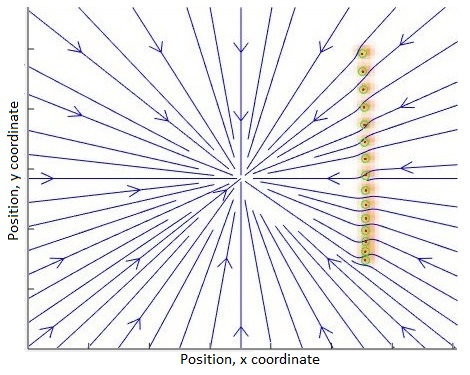
\includegraphics[width=7cm]{img/influence_small_GP.jpg}
        \caption{Influence of the correction\\\hspace{0cm}with a low length-scale}
        \label{low_influence}
    \end{minipage}
    \begin{minipage}{0.5\linewidth}
      \centering
      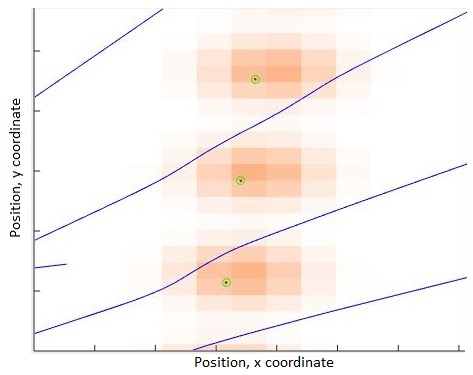
\includegraphics[width=7cm]{img/influence_small_GPzoomed.jpg}
      \caption{Influence of the correction\\\hspace{0cm}with a low length-scale zoom}
      \label{low_influence_zoom}
    \end{minipage}\hfill
\end{figure}


When zooming (and playing with hyper-parameters for more clarity) the effect from two neighbor training points can be smaller than what is necessary and some holes appears in the influence. It results in a trajectory that goes through the correction, see \autoref{eg_going_through}.\\

\begin{figure}[H]
\centering
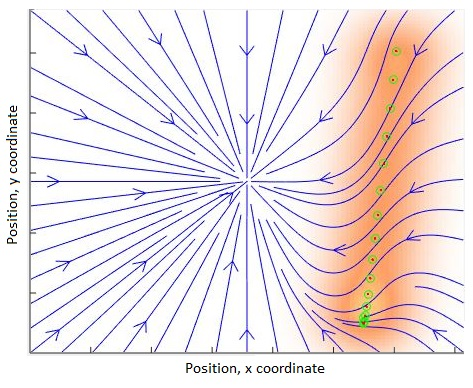
\includegraphics[width=10cm]{img/gpr_fail_thatswhy.jpg}
\caption{Example of a trajectory going through the correction.}
\label{eg_going_through}
\end{figure}

This particular problem mostly happens when training points are far from each other (and when testing it on the real robot, the situation appears quite often which makes this problem important to resolve).

The correction is interpolated into a continuous curve, so one solution would be to generate linearly spaced new interpolated data, and provide it to the GPR. However, to avoid the problem, a lot of data should be generated, which would make explode the computational cost (see quantitative analysis \autoref{booooom_explosion!}).\\
Because of the slow GPR (using in real time), there are no numeric possible solutions. But an analytical one could be possible, adapting the GPR to work with a continuous representation of the data.


%section 3 : adaptation of discrete to continuous GPR --------------------
\subsection{Adaptation of continuous GPR}

We will propose in this part a new form of GPR which will take instead of training discrete points, a continuous curve. The aim will be to drastically reduce the computational cost and increase the robustness (see \autoref{eg_going_through} problem). It will be done by selecting a particular covariance function that annihilates influence of all the curve but one points and so getting rid of the matrix inversion.

\subsubsection{Continuous input curve for GPR}

The main difference between a discrete GPR and a continuous GPR is that the training data will be a continuous curve. This curve $C$ is parametrized by a t-value $t\in [0,1]$ and allows the access of any point on the curve for a defined $t$, $c(t) \in \real^D$.\\
In our case, the continuous curve will be the correction (as extracted from a demonstration in \autoref{section_2}) interpolated into a spline (as shown in \autoref{section_3}).

\subsubsection{Curve based covariance function}

The key of our regression is the covariance function. Let $x' \in \real^D$ be a point of the curve C such as $x'=c(t')$ and $x^*$ a testing point. The covariance function is defined by:

\begin{equation}
  \label{equ_covardef}
  k(\vecc x', \vecc x^*) = exp(-(\vecc x^* - \vecc x')^T\mat \Lambda(\vecc x') (\vecc x^* - \vecc x'))
\end{equation}
where $\mat \Lambda(\vecc x') \in \real^{D \times D}$ is a metric that depends on the curve $C$ and the point $\vecc x'$. Let $\vecc e_t'$ denote the tangent vector of $C$ at $\vecc x'$. Then, $\mat \Lambda$ is defined as:

\begin{equation}
  \label{equ_lambdadefinition}
  \mat \Lambda(\vecc x') =
  \begin{bmatrix}
    \vecc e_t' & \hdots & \vecc e_D
  \end{bmatrix}
  \text{diag}([\lambda_1,\hdots, \lambda_D])
  \begin{bmatrix}
    \vecc e_t' & \hdots & \vecc e_D
  \end{bmatrix}^T
\end{equation}
where the vectors $[\vecc e_t', \hdots, \vecc e_D]$ constitute an orthonormal basis for $\real^D$. 

\subsubsection{Continuous GPR}

With \autoref{equ_lambdadefinition}, by increasing $\lambda_1$ towards infinity, the covariance function $k(x', x^*)$ tends to zero and $x^*$ satisfying $(\vecc x^* - \vecc x')^T\vecc e'_t \neq 0$, i.e for any testing point in the space which is aligned to the normal of the tangent of the curve at $x'$, the covariance function will go to 0 and the matrix \mat K in \autoref{equ_covariancetrainingdata} becomes diagonal. This means that \autoref{equ_mustrar} become:

\begin{equation}
  \label{equ_mustartreduce}
    \vecc \mu^* = \vecc k^{*T} \text{diag}\left(\left[\frac{1}{k(\vecc x_1,\vecc x_1)+\sigma_n^2},\hdots,\frac{1}{k(\vecc x_N,\vecc x_N)+\sigma_n^2}\right]\right)\vecc y
\end{equation}
\\

Assuming that $\lambda_1$ is large and $x^*$ is aligned to the normal of the tangent of the curve at the point $x'$, \emph{there is only one non-zero element in } $\vecc k^*$, it is $x'$. \autoref{equ_mustartreduce} can be simplified to:

\begin{equation}
  \label{eq_mustartreduce2}
    \vecc \mu^* = \frac{k(\vecc x',\vecc x^*)}{k(\vecc x',\vecc x') + \sigma_n^2} y'
\end{equation}
\\

Since we only have to compute the kernel with a single point ($x'$), as long as we can find this point fast enough we reduce an $N \times N$ matrix inversion to $1 \times 1$. We will see that $x'$ is simply the closest point of $x^*$ on the curve. It will be the focus of the next section.

\subsubsection{Continuous GPR implementation}

The continuous GPR makes computation quite fastly and easily by looking at \autoref{eq_mustartreduce2}. However this equation needs $x'$ which is the point on the curve where the normal of the tangent is aligned to the testing point $x^*$. This point is the closest point of $x^*$ on the curve, see \autoref{normal_curve}.\\

\begin{figure}[H]
\centering
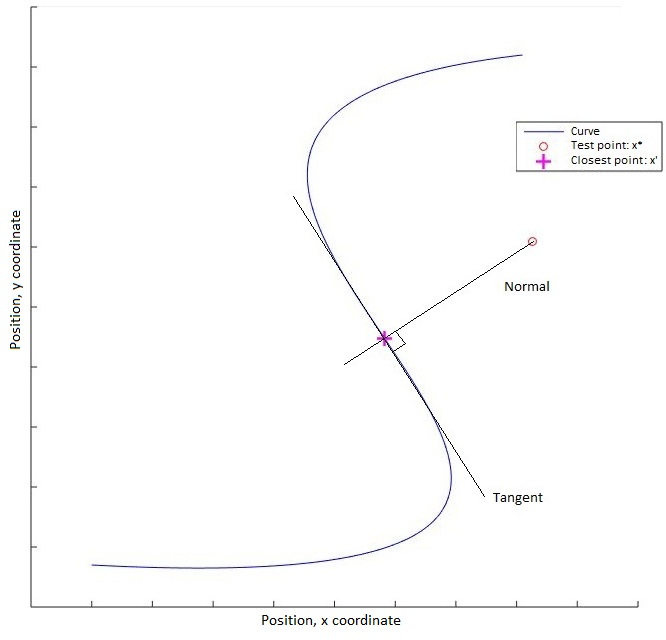
\includegraphics[width=13cm]{img/normal.jpg}
\caption{The closest point is the one which has an aligned normal.}
\label{normal_curve}
\end{figure}


For the continuous GPR implementation, an algorithm that searchs for the closest point of a testing point in the space on a continuous curve is required.

%section 4 : Distance --------------------
\clearpage
\subsection{Distance Algorithm}

For the continuous GPR adaptation, a distance algorithm is needed. This algorithm has to compute the closest distance from a point (which is anywhere in the space) on the correction (which is a continuous curve).

\subsubsection{Brute force}

Brute force is a well-known algorithm, not made for optimal-computational cost but easy to implement.\\
It works by first choosing a fix number of points on the curve which are equally distant. Those points are the interpolated points (compute by the continuous curve), they are not the knot points (knot points are not necessarily linearly spaced, with interpolated point it's possible to get any point anywhere and how much we want). Then the distance is computed for each of the interpolated points. The closest one is the closest point (see Algorithm \autoref{bf_algo}).

\begin{figure}[H]
\centering
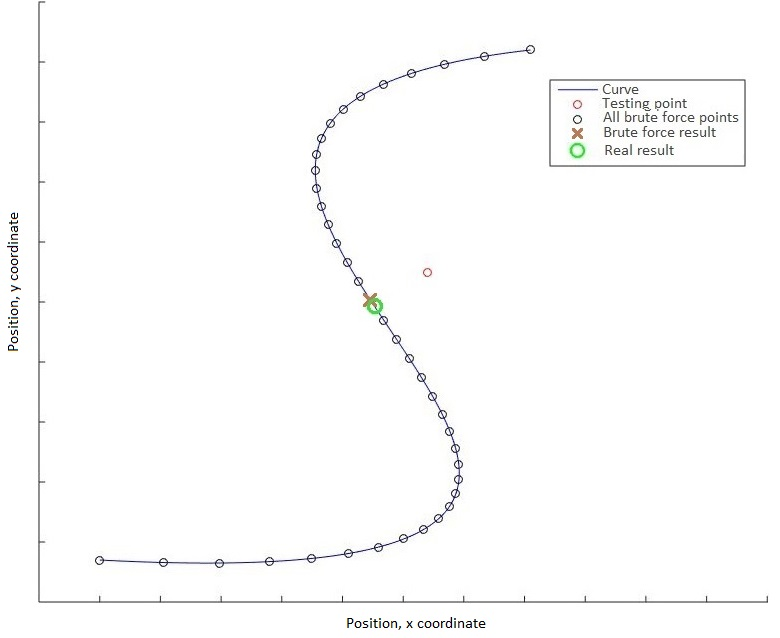
\includegraphics[width=13cm]{img/brute_force.jpg}
\caption{Example of brute force algorithm with 40 points.}
\end{figure}

\begin{algorithm}[H]
  \caption{brute force search}
  \label{bf_algo}
  \begin{algorithmic}

      \STATE input : continuous correction: $x_{xyz}(t)$, testing point: $x_{xyz}^*$
      \STATE

      \STATE $N = 10000$  \#N can be given as an input
      \STATE $indices = linearly\_spaced(0,1,N)$ \#provides N linearly spaced points from 0 to 1
      \STATE $result = 0$
      \STATE

        \FOR{$i\ in\ indices$}
            \IF {$distance(x_{xyz}(i),x_{xyz}^*) < distance(x_{xyz}(result),x_{xyz}^*)$}
                \STATE $result = i$
            \ENDIF
        \ENDFOR

        \STATE
        \STATE output: the closest point: $x_{xyz}(result)$

    \end{algorithmic}
\end{algorithm}

\paragraph*{Advantage}

This algorithm is very easy to implement and gives quite accurate results.

\paragraph*{Disadvantage}

This algorithm is very heavy, takes a lot of computational cost, $ O(n) $ where n is the number of points, and it's precision directly depends on the number of points.
Typically, a good number of point for this application is $ n=10000 $, which takes too much time to compute.

\subsubsection{Dichotomy}

This algorithm, also called Bisection-method, is based on selecting successively sub-intervals and testing the distance of the boundary points. Sub-intervals are selected by choosing the middle of the latest sub-intervals until converging to the good point (see Algorithm \autoref{dy_algo}).\\

Another application for this algorithm is searching a value in an ordered array, by taking the middle of the sub interval until reaching the value or the place where the value should be.

\begin{figure}[H]
\centering
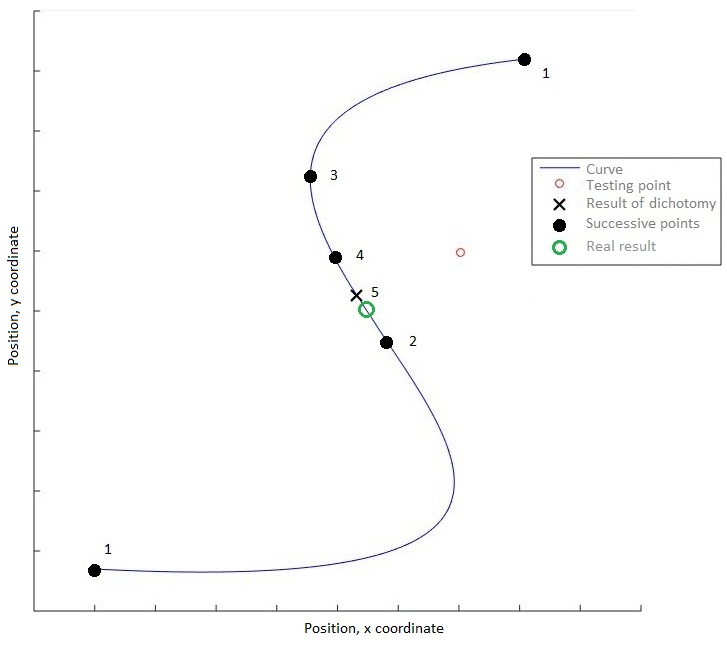
\includegraphics[width=13cm]{img/dichotomy.jpg}
\caption{Example of dichotomy algorithm with 5 iterations.}
\label{dichotomy_ex}
\end{figure}

In this example (\autoref{dichotomy_ex}), we can see that this method converges very quickly to the result, even if one or two more computations would have given a good precision in this example.

\begin{algorithm}[H]
  \caption{Dichotomic search}
  \label{dy_algo}
  \begin{algorithmic}

      \STATE input : continuous correction: $x_{xyz}(t)$, testing point: $x_{xyz}^*$
      \STATE

      \STATE $N = 40$ \#N can be given as an input
      \STATE $sublimit1 = 0$
      \STATE $sublimit2 = 1$ \#sublimit1-2 are the boundary of the sub-interval
      \STATE

        \FOR{$i\ from\ 1\ to\ N$}
            \IF {$distance(x_{xyz}(sublimit1),x_{xyz}^*) < distance(x_{xyz}(sublimit2),x_{xyz}^*)$}
                \STATE $sublimit2 = (sublimit1+sublimit2)/2$ \#sublimit2 is further, need to be changed
            \ELSE
                \STATE $sublimit1 = (sublimit1+sublimit2)/2$ \#sublimit1 is further, need to be changed
            \ENDIF
        \ENDFOR

        \STATE
        \STATE output: the closest point: $x_{xyz}(sublimit1)$

    \end{algorithmic}
\end{algorithm}

\paragraph*{Advantage}

This algorithm can be very precise, it has a very low computational cost, $ O(n) $ where $n$ is the number of iteration (in this implementation $ O(n) $ but with binary search it is $ O(log_2(m)) $ where m is the length of the array). Typically, for this kind of application you could choose $ n = 40 $.\\
Even if the computational cost is the same for the brute force algorithm, it is said here to be low because of the small required value of $n$.

\paragraph*{Disadvantage}

This algorithm can be precise, but can also give a completely wrong result, it detects only local minimal which is a problem, the minimal distance point of all the curve is needed here, see \autoref{dicho}.

\begin{figure}[H]
\centering
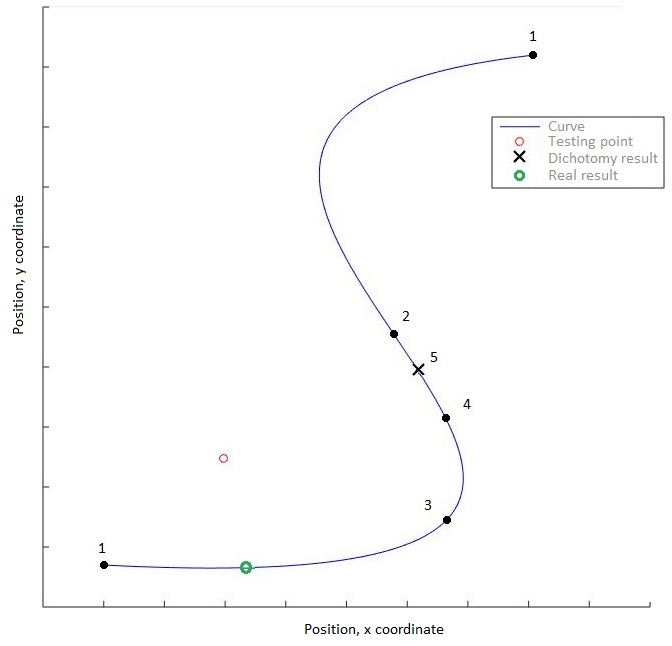
\includegraphics[width=13cm]{img/dichotomy_bad.jpg}
\caption{Example of dichotomy algorithm with 5 points which fail.}
\label{dicho}
\end{figure}

When testing this method, we figure out that this problem occurs quite often.

\newpage
\subsubsection{Analytic solution} \label{GPR_ANALYTIC_SUBSUB}

The continuous curve is a spline defined by many cubic splines on each axis in the following form (the robot environment is in 3 dimensions so there are 3 splines parametrized by a t-parameter, $t\in[0,1]$)\\

\begin{equation}
  \begin{split}
    f_x(t) = a_x t^3+b_x t^2+c_x t+d_x\\
    f_y(t) = a_y t^3+b_y t^2+c_y t+d_y\\
    f_z(t) = a_z t^3+b_z t^2+c_z t+d_z
  \end{split}
\end{equation}

\paragraph*{Maths}

The distance from a point $(x^*, y^*, z^*)$ to another point on the curve is:\\
$$ distance(t) = \sqrt{(x^* - f_x(t))^2 + (y^* - f_y(t))^2 + (z^* - f_z(t))^2} $$
\\
The minimal distance is found by deriving:\\
$$ \frac{d(distance(t))}{dt} = \frac{-2f_x'(t)(x^* - f_x(t)) - 2f_y'(t)(y^* - f_y(t)) - 2f_z'(t)(z^* - f_z(t))}{\sqrt{(x^* - f_x(t))^2 + (y^* - f_y(t))^2 + (z^* - f_z(t))^2}} = 0 $$
\\
$$ \frac{d(distance(t))}{dt} = -2f_x'(t)(x^* - f_x(t)) - 2f_y'(t)(y^* - f_y(t)) - 2f_z'(t)(z^* - f_z(t)) = 0 $$
\\
We focus now on $ S_x = -2f_x'(t)(x^* - f_x(t)) $ because the calculus are the same for dimension x, y and z.\\
We know that:\\
$$ f_x(t) = a_x t^3+b_x t^2+c_x t+d_x $$
$$ f_x'(t) = 3a_x t^2+2b_x t+c_x $$\\
so:\\
$$ S_x = -2f_x'(t)(x^* - f_x(t)) = -2(3a_x t^2+2b_x t+c_x)(x^* - a_x t^3 - b_x t^2 - c_x t - d_x) $$\\
After factorization:\\
$$ S_x = 6a_x^2t^5 + 10a_xb_xt^4 + (8a_xc_x + 4b_x^2)t^3 + (6a_xd_x + 6b_xc_x - 6a_xx^*)t^2 + (4b_xd_x + 2c_x^2 - 4b_xx^*)t + (2c_xd_x - 2c_xx^*) $$
$$ S_x + S_y + S_z = 0 $$\\

Since there are 5 roots to this polynomial, we compute the solution by removing complex roots, and finally taking the closest root of the few remaining.

\paragraph*{Result interpretation}

This method is very powerful, as an analytically algorithm, its computational cost is low and constant and, by definition, the most accurate possible.\\

The result will be the absolute closest point on the curve to the testing point, but it will not necessarily be in the interval $t\in[0,1]$, depending on the testing point. This is not a problem, it is very simple to test if the result point is in the interval, and if not, it means that the trajectory is not going through the given correction, see \autoref{analytic_fail}.

\begin{figure}[H]
\centering
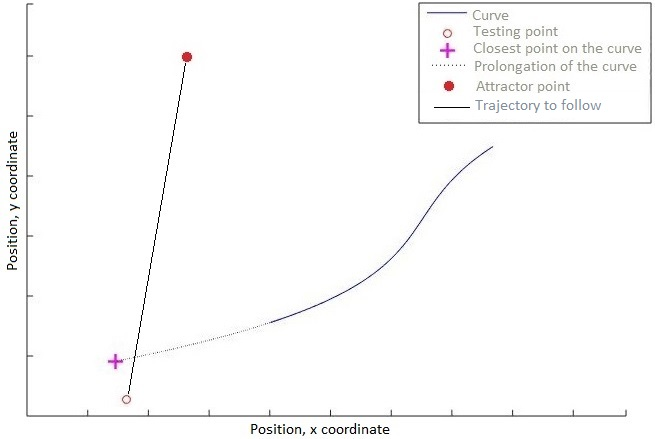
\includegraphics[width=10cm]{img/analytic_fail.jpg}
\caption{Example of a trajectory which is not going through the correction and therefore shouldn't be influenced by the curve.}
\label{analytic_fail}
\end{figure}

In this particular case, the testing point is set on purpose somewhere where the straight trajectory wouldn't cross the correction, so the trajectory from the testing point to the attractor shouldn't be influence by the correction. We can see that the result of the closest point algorithm returns a value (pink +) that is not on the correction, this is the absolute closest point of the analytic curve. This result is not a problem, indeed it's very easy to test if the result is located on the correction and if not, the point is considered to not be influenced by the correction.

\begin{figure}[H]
\centering
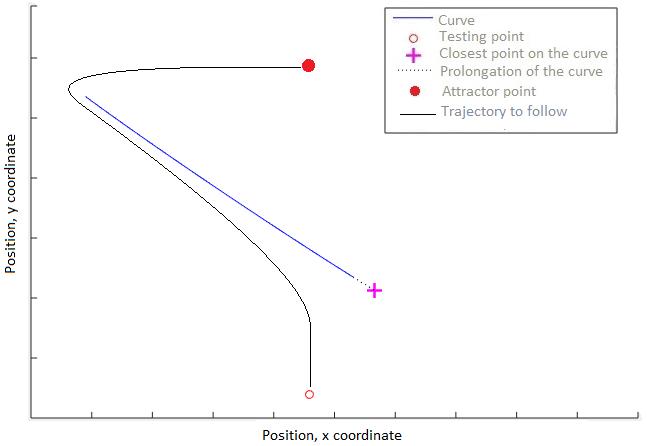
\includegraphics[width=10cm]{img/analytic_fail2.png}
\caption{Example of a trajectory which was going through the correction but still out of the interval.}
\label{analytic_fail_2}
\end{figure}

In this example \autoref{analytic_fail_2}, the testing point is set on purpose somewhere where the straight trajectory would cross the correction but where the distance-point algorithm would return a value out of the correction. It's also not a problem, as we can see in black, the trajectory goes forward until the closest point reach the correction, and the GPR will have an effect before that the trajectory cross the correction.\\

For its constant computational cost and very good accuracy, the analytic algorithm will be chosen for the continuous Gaussian process regression computation. This algorithm will be used in the quantitative analysis.\\

The correction is usually composed by many splines which is composed by many polynomial functions, therefore, the algorithm will be executed many times. One closest point is compute per polynomials functions and the final closest point is the closer one.

\clearpage
\subsection{Analysis}

To analyze the result of this adapted algorithm, some tests will be done, all the time by comparing the discrete and the continuous Gaussian Process Regression. \\
First we will analyze the accuracy by checking if the new algorithm return a good result with a low number of training points.\\
Then we will analyze the computational cost by varying the number of testing points and the number of training points.

\subsubsection{Accuracy of continuous Gaussian Process Regression}

To compare the influence of the continuous and discrete GPR, we took a correction made by 3 points, and tested its influence on some testing points.

\begin{figure}[H]
\centering
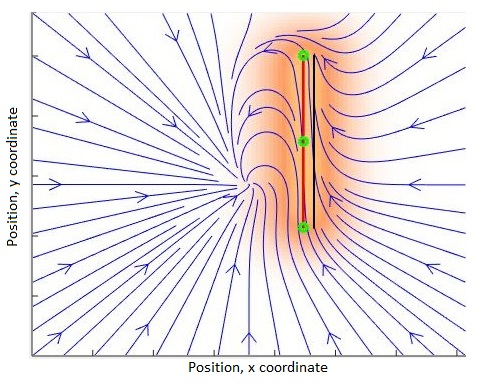
\includegraphics[width=10cm]{img/gp_test.JPG}
\caption{Test for continuous and discrete GPR.}
\label{quan_gpr_1}
\end{figure}

For this test (see \autoref{quan_gpr_1}), 3 training discrete points were taken (green circle), a spline was computed (in red) that will be the training continuous data and many testing points were chosen on a parallel line (in black) so that the influence of the curve on the testing points will be very clear.

\begin{figure}[H]
    \begin{minipage}[b]{0.5\linewidth}
        \centering
        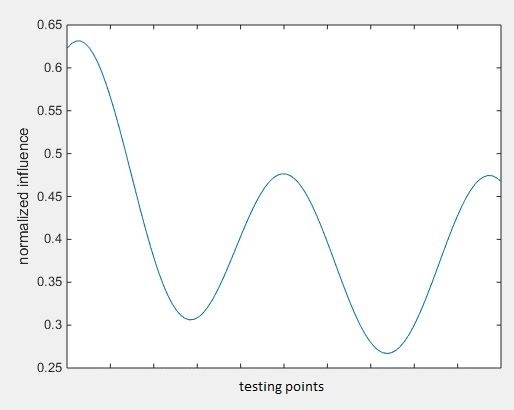
\includegraphics[width=0.90\textwidth]{img/discrete_gp_norm.jpg}
        \caption{Graph of the normalized influence of the discrete Gaussian process on the test points.}
        \label{discrete_gp_test}
    \end{minipage}
    \begin{minipage}[b]{0.5\linewidth}
        \centering 
        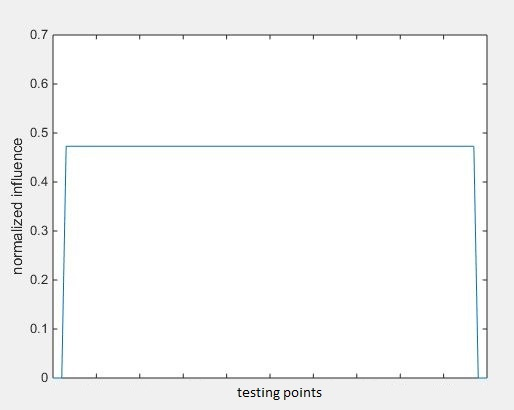
\includegraphics[width=0.90\textwidth]{img/continuous_gp_norm.jpg}
        \caption{Graph of the normalized influence of the continuous Gaussian process on the test points.}
        \label{continuous_gp_test}
    \end{minipage}\hfill
\end{figure}

As we can see on \autoref{discrete_gp_test}, only the 3 training points influence the result, that's why there are 3 squared-exponential in the graph. Typically a trajectory could go through the correction when the influence is the lowest (see \autoref{eg_going_through}).
On \autoref{continuous_gp_test}, the influence is constant, no trajectory will be able to cross the correction. This is exactly what the continuous Gaussian Process Regression was developed for.\\

This test was done to prove that the influence $|GP|$ is not local to the knot points of the correction but is a general influence of the entire correction curve, due to the continuous GPR.

\subsubsection{Computation time}

To compare the computational cost of both algorithms, first we varied the number of test points and then the number of training points.\\
Algorithms were simulated on a computer, the time was numerically computed. The same system as below (\autoref{quan_gpr_1}) is used.

\paragraph*{Testing points number variation}

First, the computationnal cost of the GPRs algorithms are tested by having the number of testing point varying. As in \autoref{quan_gpr_1}, there is a vertical line on which many testing points linearly spaced were computed.

\begin{figure}[H]
\centering
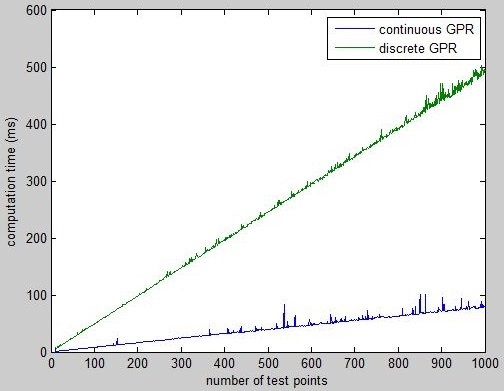
\includegraphics[width=11cm]{img/analysis_time_both.jpg}
\caption{Graph of computational time for GPR algorithms. Testing points vary with 3 training points.}
\label{booooom_explosion!}
\end{figure}

Both algorithm computational times increase linearly, but for the continuous algorithm, it's increasing slower and the values are almost 10 times smaller.

\paragraph*{Training points number variation}

The computationnal cost of the GPRs algorithm are tested by having the number of training point varying. As in \autoref{quan_gpr_1}, there is a vertical line on which many training points linearly spaced were computed. Another parameter was tested here, the smoothing parameter. Indeed, while using the robot to get data, the robot is sending a lot of data very fastly and the algorithm gets very quickly slow. That's why a decimation algorithm has been used to have a lower number of training point but still a good representation of the correction.\\

A coefficient of decimation called smoothing was used, it works very simply: if equals to 1, we keep all the data, if equals to 0.5, we keep half of the data (every two points, one is removed) and the same kind of behavior for every values between 0 and 1.

\begin{figure}[H]
    \begin{minipage}[b]{0.5\linewidth}
        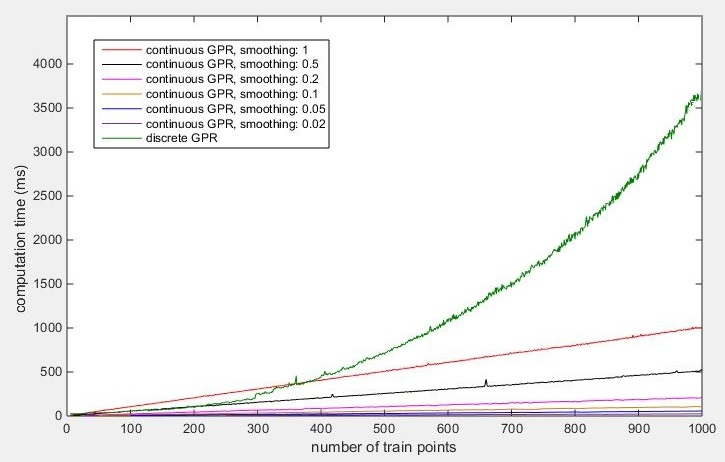
\includegraphics[width=8cm]{img/all_curve_training_analysis.jpg}
        \caption{Graph of computational time for discrete and continuous GPR algorithms on 100 testing points with a smoothing of 1, 0.5, 0.2, 0.1, 0.05, 0.02.}
        \label{gp_test_train}
    \label{bezier_example}
    \end{minipage}
    \begin{minipage}[b]{0.5\linewidth}
        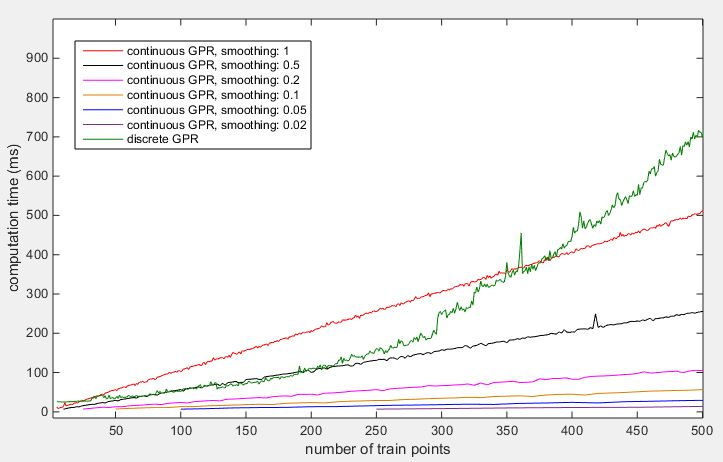
\includegraphics[width=8cm]{img/all_curve_training_analysis_500.jpg}
        \caption{Zoom on the 500 first points of \autoref{gp_test_train}.\\\hspace{0cm}\\\hspace{0cm}}
        \label{gp_test_train_500}
    \end{minipage}\hfill
\end{figure}

% \begin{figure}[H]
% \centering
% 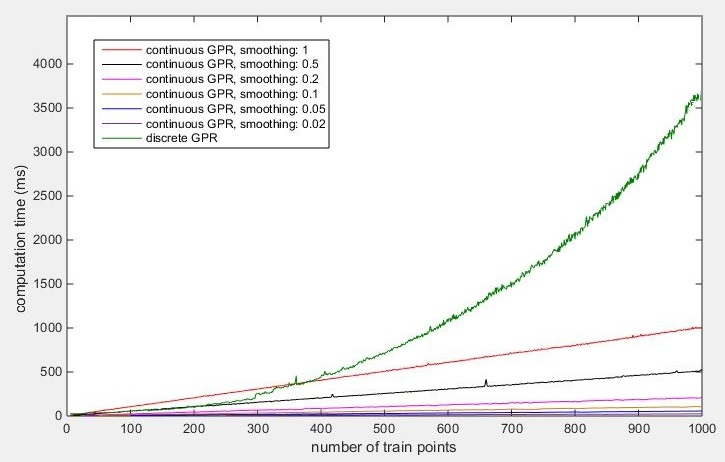
\includegraphics[width=16cm]{img/all_curve_training_analysis.jpg}
% \caption{Graph of computational time for discrete and continuous GPR algorithms on 100 testing points with a smoothing of 1, 0.5, 0.2, 0.1, 0.05, 0.02.}
% \label{gp_test_train}
% \end{figure}

\begin{figure}[H]
\centering
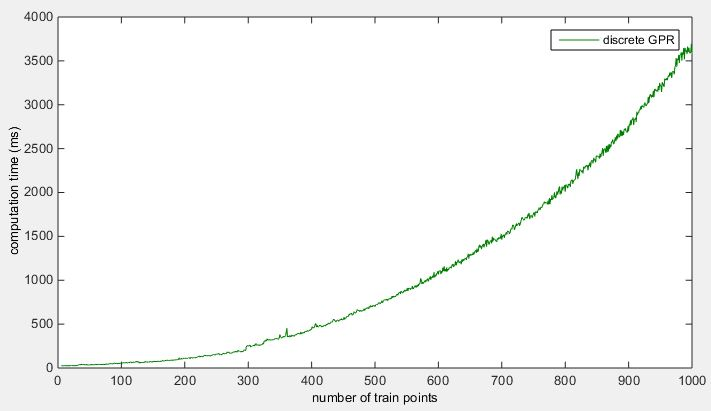
\includegraphics[width=0.95\textwidth]{img/discrete_curve_training_analysis.jpg}
\caption{\autoref{gp_test_train} with only the discrete GPR curve.}
\label{gp_test_train_only_d}
\end{figure}

\begin{figure}[H]
\centering
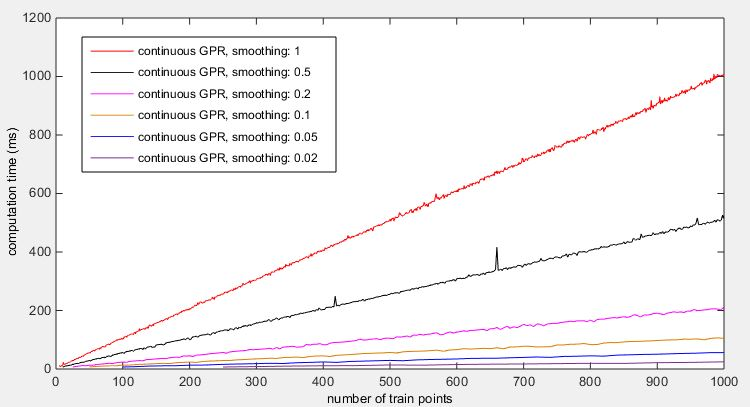
\includegraphics[width=0.95\textwidth]{img/all_wd_curve_training_analysis.jpg}
\caption{\autoref{gp_test_train} with only the continuous GPR curves.}
\label{gp_test_train_all_wd}
\end{figure}


On \autoref{gp_test_train_only_d} we can see the computation time of the discrete GPR algorithm vary quadratically.\\
The general shape of the curves of the continuous algorithm on \autoref{gp_test_train_all_wd} are linear. Indeed, if there are many training points, there will be many cubic splines (one between each training point), so the distance algorithm will have to compute the minimal distance point on each cubic splines, and then took the closest one. Even if this algorithm has a constant computational cost for a single cubic splines, the continuous GPR will take linearly more times to be compute. The most the smoothing goes to zero, the faster it will be to compute the continuous GPR.\\

All those tests were done on a computer, the computational time is not a perfectly linear, quadratic or constant signal because there are always many tasks running at the same time which affects randomly the time values (indeed, we are measuring in milliseconds scale, it is very sensitive). Tests were done in the best possible conditions with the least amount of parallel tasks possible to minimize the problem.\\

Those analyses show that the continuous GPR gives better result for high number of training points, but the standard GPR is better with a low number of training points. This is directly linked to the inversion of the $N \times N$ matrix (if N is low the inversion will be fast) and the constant computationnal cost of the analytic distance algorithm.

